\chapter{Hardware Implementation}

% **************************** Define Graphics Path **************************
\ifpdf
    \graphicspath{{Chapter3/Figs/Raster/}{Chapter3/Figs/PDF/}{Chapter3/Figs/}}
\else
    \graphicspath{{Chapter3/Figs/Vector/}{Chapter3/Figs/}}
\fi

The following sections shows us an overview about the hardware implementation of the Invariant Observer Design.
At first we get a description about the hardware platform on which the observer runs and some details
about the synthesis tools.
At the end of this chapter, there comes a design view about the synthesized hardware and a discussion about 
the design steps.
\section{Hardware Platform for a Prototype}
The Invariant Observer is synthesized on a Field Programmable Gate Array(FPGA),on this platform it was possible to get an insight
about the runtime behaviour and to see the observers in action. 
The FPGA Board that was used for the simulations is a \textbf{DE2-115} Board from ALTERA\cite{altera1}.
This FPGA Board is ideal to illustrate fundamental concepts and advanced designs,and it gives us a possibiliy
to meet the necessary real-time requirements we need. The DE2-115 is equipped with a \textbf{Cyclone IV EP4CE115F29} 
FPGA Chip and it is powerful enough to emulate a CPU(Nios).In \cite{RTFMBJ13} this Fpga board was used for performance studies,besides other FPGA's,
so it was logical to use a similar environment.
The Board has an onboard oscillator of 50 Mhz,and with the use of a Phase Locked Loops(PLL) it is possible to increase the frequency for tests.
In the following section we will see how the increase of the frequency changes the design on Register Transfer level(RTL) and why bad design decisions 
can influence the maximal speed of the design. In Appendix~\ref{appendix:3:1} there is an schema illustration about the components of that FPGA board.


\section{Synthesis and Design}
This section gives us an overview about the synthesis tool and details about the Register Transfer Level design view.
An interesting part in this section is to see how the synthesis tool creates hardware structures based on the code of the
Observer VHDL implementation.\newline
For synthesis and compilation of the observer vhdl code ,the \textbf{Altera Quartus II Version 12.1 Build 177 Full Version} was used.
\subsection{Design View on the Register Transfer Level}
In Quartus II ,after compilation of the design and after creation of the netlists,there is a tool,named \textbf{RTL Viewer}, which shows how
the components of the design will be created on Hardware Platform. It is an abstract view on the \textbf{Register Transfer Level}.
This tool can be very handy if you want to see how the hardware should look like. Based on the illustration of the hardware,some decisions can
be reconsidered in the meaning of the performance. \newline
Figure~\ref{fig:test:only:50:obs0} is a hardware plan of a single observer stage m=1,which is modeled as a single Observer with input frequency of 50Mhz.
How the test system was modeled for that case,will be discussed in the next chapter.
One important fact,that have to be considered,is that the signal path from the beginning of the observer entity until the end should be as short as possible.
Let's overview some important design decisions.\newline
The maximum frequency of the whole system is determinded by the longest path of the design. This results that the performance of a system is determined by the maximum frequency
it can be driven. It is logical that,at every entity in the netlist,the path should be as short as possible.
The performance maximum can be computed by the Quartus Tool named \textbf{TimeQuest Timing Analyzer},which gives estimations about the maximum frequency of the design.
The ĺongest signal path of the design is indicated by the \textbf{worst case path} in the tool. \newline
The first version of the observer stage had a low performance niveau. This version is illustrated in the Appendix~\ref{fig:version:one:obs}.
The TimeQuest Timing Analyzer consider some uncertainties for the performance estimations.A Fpga have to operate in a continuum of conditions. These conditions 
include the die junction temperature,which varies.Commercial parts have a range of 0°C to 85°C and industrials a bigger range.A second condition aspect is voltage supply level.



\begin{figure}[]
\centering
%\hspace{3.0cm}
%\vspace{-5cm}
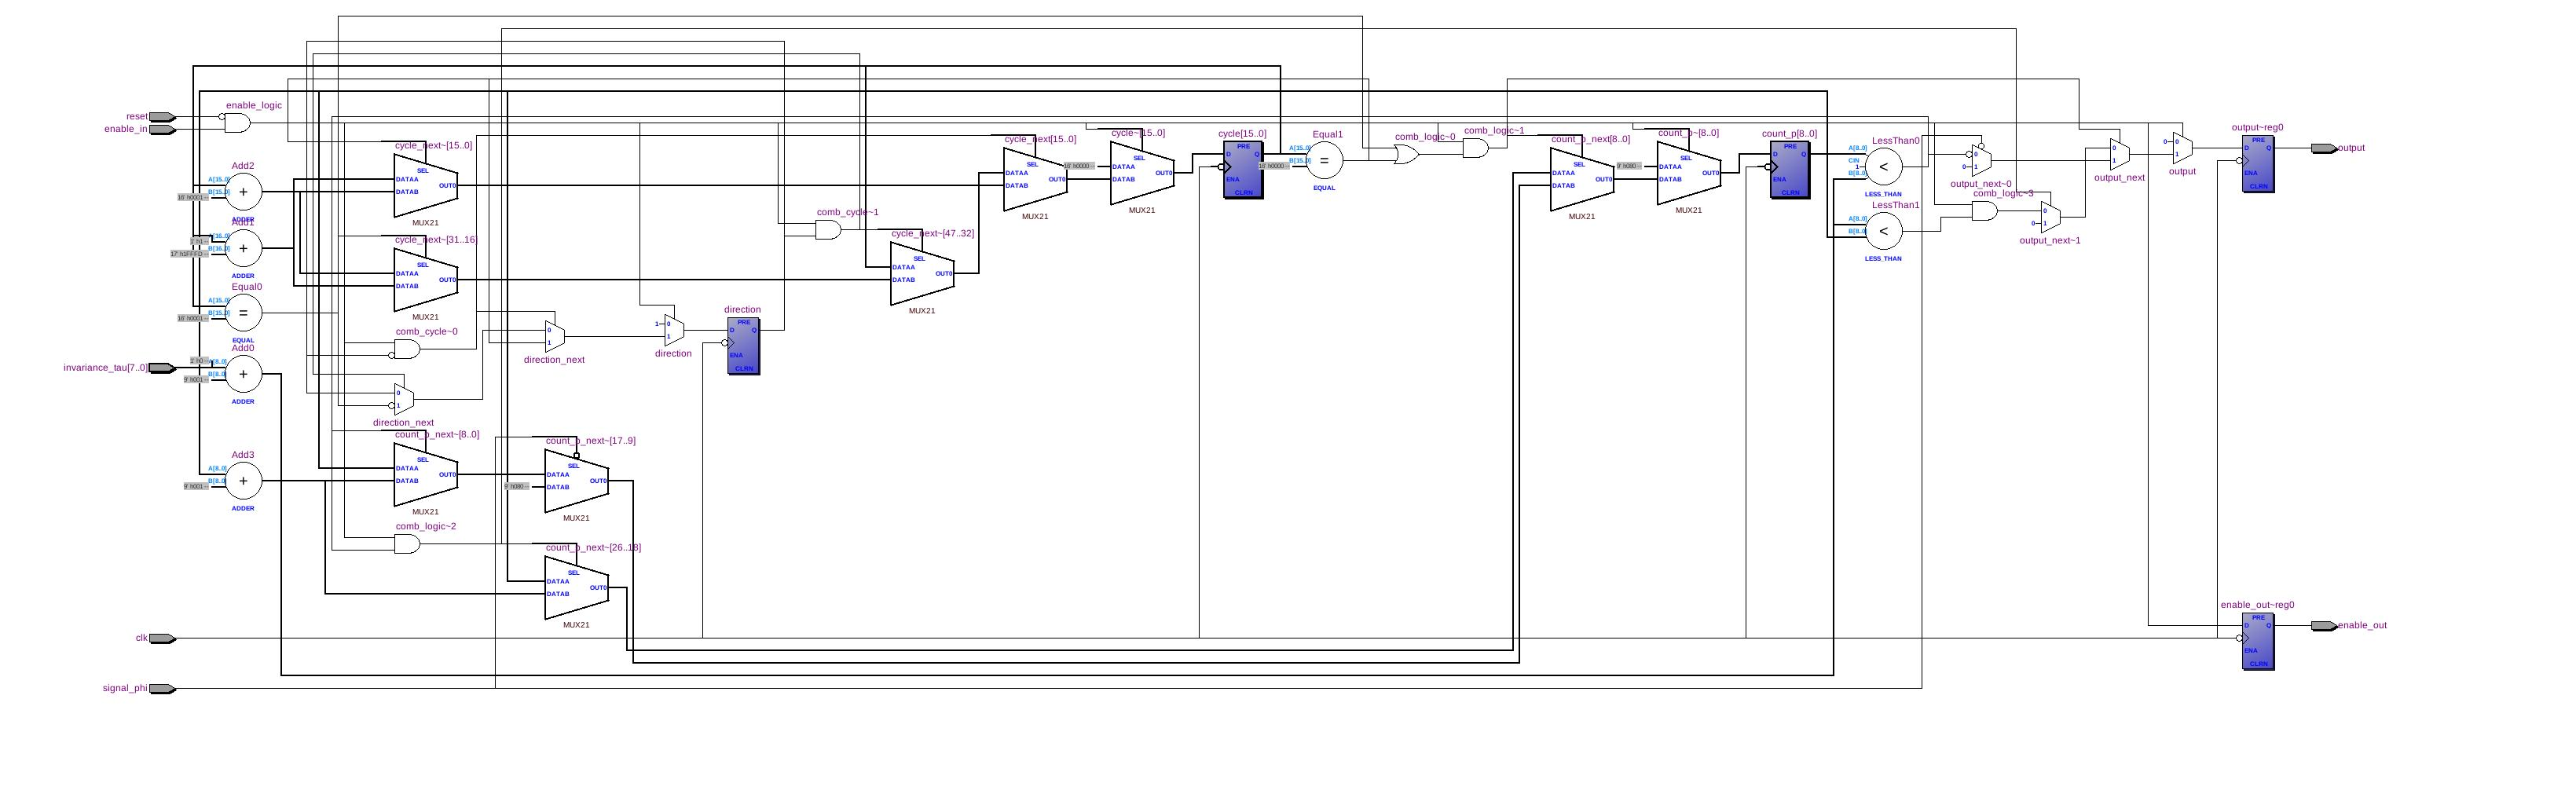
\includegraphics[width=650px,height=300px,angle=-90]{../../pictures/22.02.2014/onlyObserver/OBS_50M.jpg}
\caption[RTL View of Observer 0 with clock 50Mhz]{Shows a RTL View of a single observer stage with input clock of 50Mhz}
\label{fig:test:only:50:obs0}
\end{figure}


\begin{figure}[]
\centering
%\hspace{3.0cm}
%\vspace{-5cm}
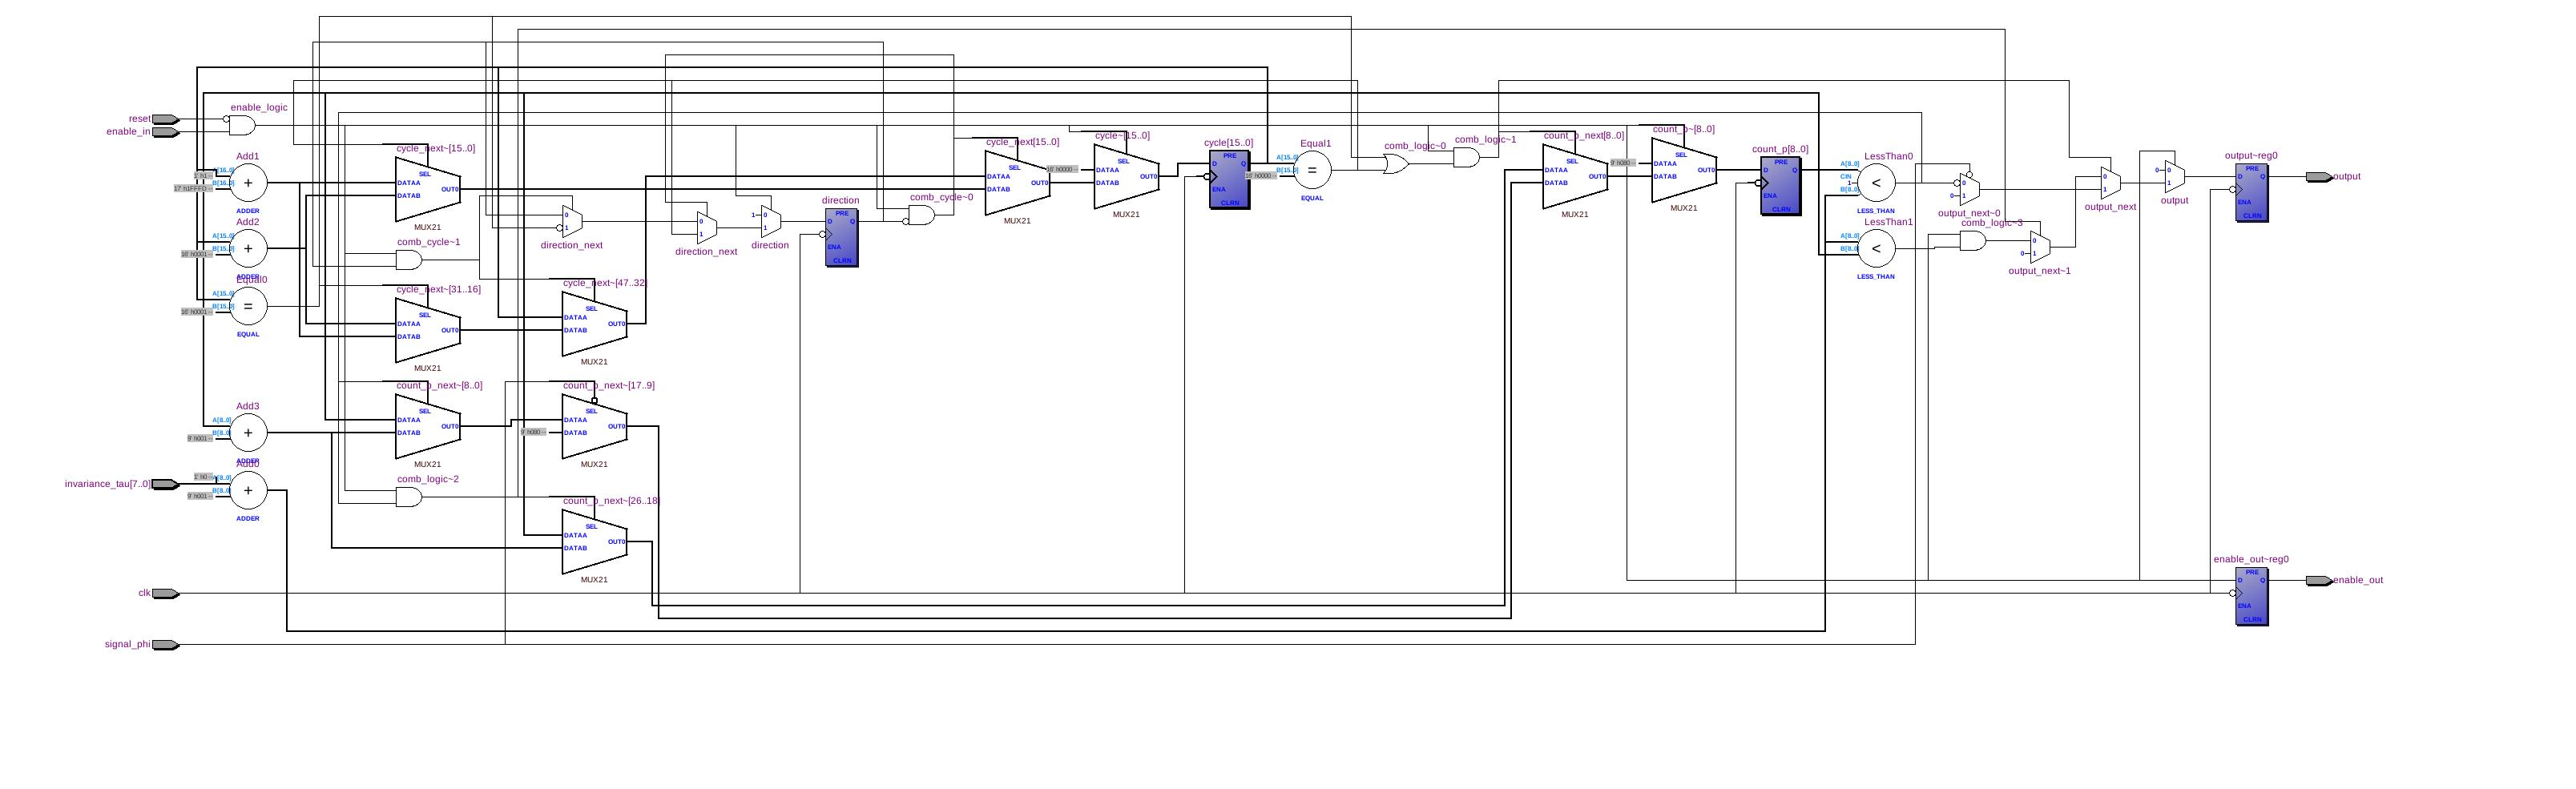
\includegraphics[width=650px,height=300px,angle=-90]{../../pictures/22.02.2014/onlyObserver/OBS_150M.jpg}
\caption[RTL View of Observer 0 with clock 150Mhz]{Shows a RTL View of a single observer stage with input clock of 150Mhz}
\label{fig:test:only:50:obs0}
\end{figure}

\newpage
The timing analyzer shows estimations for three cases
\begin{enumerate}
\item Slow 1200mv 85°C model
\item Slow 1200mv 0°C model
\item Fast 1200mv 0°C model
\end{enumerate}
\section{Troubles and Mistakes in the development}
